%%%%%%%%%%%%%%%%%%%%%%%%%%%%%%%%%%%%%%%%%%%%%%%%%%%%%%%%%%%%
%%  Presentation of Bachelor thesis. 
%%  A network model of the neocortex accounting for its laminar structure
%%  Friedrich Schuessler
%%  September 2015

\documentclass[xcolor=x11names,compress]{beamer}
\usepackage[utf8]{inputenc} 
\usepackage[T1]{fontenc}
\usepackage{cmbright}

%% General document %%%%%%%%%%%%%%%%%%%%%%%%%%%%%%%%%%
\usepackage{graphicx}
\usepackage{caption}  
\usepackage{subcaption}     % subfloats

\usepackage{tikz}

\usepackage[style=authoryear]{biblatex}
\usetikzlibrary{decorations.fractals}
%%%%%%%%%%%%%%%%%%%%%%%%%%%%%%%%%%%%%%%%%%%%%%%%%%%%%%


%% Beamer Layout %%%%%%%%%%%%%%%%%%%%%%%%%%%%%%%%%%
\useoutertheme[subsection=false,shadow]{miniframes}
\setbeamerfont{title like}{shape=\scshape}
\setbeamerfont{frametitle}{shape=\scshape}

\setbeamercolor*{lower separation line head}{bg=DeepSkyBlue4} 
\setbeamercolor*{normal text}{fg=black,bg=white} 
\setbeamercolor*{alerted text}{fg=red} 
\setbeamercolor*{example text}{fg=black} 
\setbeamercolor*{structure}{fg=black} 

\usenavigationsymbolstemplate{}
\setbeamercolor*{palette tertiary}{fg=black,bg=black!10} 
\setbeamercolor*{palette quaternary}{fg=black,bg=black!10} 

\setbeamercovered{dynamic} % enable pause

\renewcommand{\(}{\begin{columns}}
\renewcommand{\)}{\end{columns}}
\newcommand{\<}[1]{\begin{column}{#1}}
\renewcommand{\>}{\end{column}}
%%%%%%%%%%%%%%%%%%%%%%%%%%%%%%%%%%%%%%%%%%%%%%%%%%
\useoutertheme{infolines} % authors, etc.
%%%%%%%%%%%%%%%%%%%%%%%%%%%%%%%%%%%%%%%%%%%%%%%%%%

\bibliography{presentation.bib}

\DeclareGraphicsExtensions{.pdf,.png,.jpg, .eps}

%%%%%%%%%%%%%%%%%%%%%%%%%%%%%%%%%%%%%%%%%%%%%%%%%%%%%
% My own definitions
\usepackage{color, colortbl}  
\definecolor{TableColor}{HTML}{A1D99B}

% Math stuff
\newcommand*\diff{\mathop{}\!\text{d}}
\newcommand*\Diff[1]{\mathop{}\!\text{d^#1}}

%%%%%%%%%%%%%%%%%%%%%%%%%%%%%%%%%%%%%%%%%%%%%%%%%%%%%%%
\begin{document}

\begin{frame}{}
\title[Neocortex]{A network model of the neocortex accounting for its laminar structure}
\author{
Friedrich Schüßler}
\date{\normalsize September 21, 2015}
%\date{\today}
\titlepage

\centering 
Supervisor: Prof. Jens Timmer
\end{frame}

\begin{frame}{Table of contents}
    \tableofcontents
\end{frame}

\AtBeginSection[]{
\begin{frame}{Table of contents}
    \tableofcontents[currentsection]
\end{frame}
}

\section{Central goals}

\begin{frame}[t]{Central goals of the thesis}
    \begin{block}<1->
        {Implement a spiking network model of the neocortex}
        \vspace{0.2cm}
        \footnotesize
        Tobias C Potjans and Markus Diesmann. \\
        The cell-type specific cortical microcircuit:
        Relating structure and activity in a full-scale spiking network model. \\
        \textit{Cerebral cortex}, 24(3): 785-806, 2014.
    \end{block}
    \vfill
    \begin{block}<2->
        {Develop a mean field theory for the neocortical model}
        \vspace{0.2cm}
        \footnotesize
        Nicolas Brunel. \\
        Dynamics of sparsely connected networks of excitatory and inhibitory spiking 
        neurons. \\
        \textit{Journal of computational neuroscience}, 8(3):183-208, 2000.
    \end{block}
\end{frame}


\section{Theory}
\label{sec:theory}


\begin{frame}{Layered structure}
    \begin{columns}[T] % contents are top vertically aligned
    \begin{column}[T]{5cm} % each column can also be its own environment
        \begin{block}{8 Populations of size $N_a$}
        \end{block}
        \vfill
        \begin{block}<2->{Synapse numbers $C_{ab}$}
        \end{block}
        \vfill
        \begin{block}<3->{External input of frequency $\nu_\text{ext}$}
        \end{block}
    \end{column}
    \begin{column}[T]{5cm} % alternative top-align that's better for graphics
        \includegraphics<1-1>[width=1.\linewidth]{../figures/diagram_pre}
        \includegraphics<2-2>[width=1.\linewidth]{../figures/diagram_conn}
        \includegraphics<3->[width=1.\linewidth]{../figures/diagram}
    \end{column}
    \end{columns}
\end{frame}

\begin{frame}{Membrane dynamics}
    \begin{columns}[T] % contents are top vertically aligned
    \begin{column}[T]{7cm} % each column can also be its own environment
    \only<1->{
        \begin{equation*}
            \tau_\text{m} \,\frac{\text{d} V_i(t)}{\text{d} t} 
                    = - V_i(t) + \frac{\tau_\text{m}}{C_\text{m}} I_i(t)
        \end{equation*}
        \begin{tabular}{>{$}p{1.0cm}<{$} l}
            V_i(t)         &  Membrane potential \\ 
            \tau_\text{m}  &  Membrane time constant \\
            C_\text{m}     &  Membrane capacity    \\
            I_i(t)         &  Input current        
        \end{tabular} \\
    }
    \vspace{1cm}
    \only<2->{
        If $V_i(t)$ reaches the threshold $\theta$:
        \begin{itemize}
            \item Spike is emitted
            \item $V_i(t) = V_r$ \quad for refractory period $\tau_\text{rp}$
        \end{itemize}
    }
    \end{column}
    \begin{column}[T]{3cm} % alternative top-align that's better for graphics
        \only<1->{
            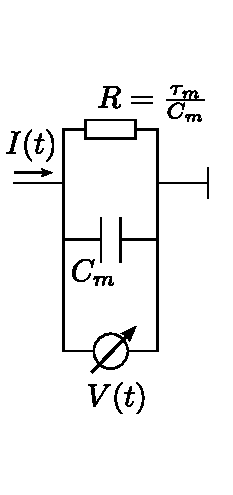
\includegraphics[height=0.7\textheight]{../figures/RC_circuit}
        }
    \end{column}
    \end{columns}
\end{frame}

\begin{frame}{Synapse dynamics}
%\only<1->{
    Single spike
    \begin{equation*}
    I_{\text{syn}}(t) = w \exp{\left(\frac{-t}{\tau_\text{syn}}\right)}	
    \end{equation*}
    \begin{tabular}{>{$}p{2.5cm}<{$} l}
        w               & Synaptic strength \\
        \tau_\text{syn} & Synaptic time constant 
    \end{tabular}
%}
%\vfill
%\only<2->{
    %Total current
    %\begin{equation*}
        %I_i(t) = 
            %\sum_j w_{ij} \sum_k 
            %\exp\left(\frac{t - t_j^k - d_{ij}}{\tau_\text{syn}}\right) 
    %\end{equation*}
    %\begin{tabular}{>{$}p{2.5cm}<{$} l}
        %d_{ij}               & Delay \\
    %\end{tabular}
%}
\end{frame}

\begin{frame}{Example}
    %\begin{columns}[T] % contents are top vertically aligned
    %\begin{column}[T]{5cm} % each column can also be its own environment
        \only<1-1>{
            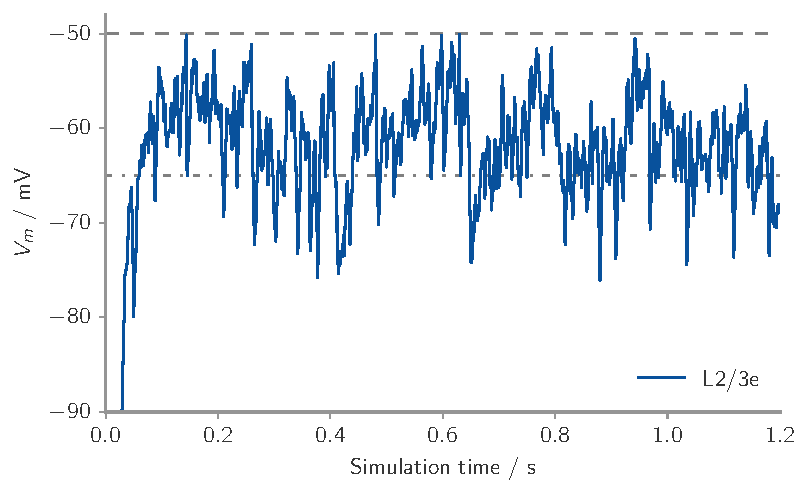
\includegraphics[height=0.8\textheight]{../figures/single_membrane_potential}
        }
        \only<2-2>{
            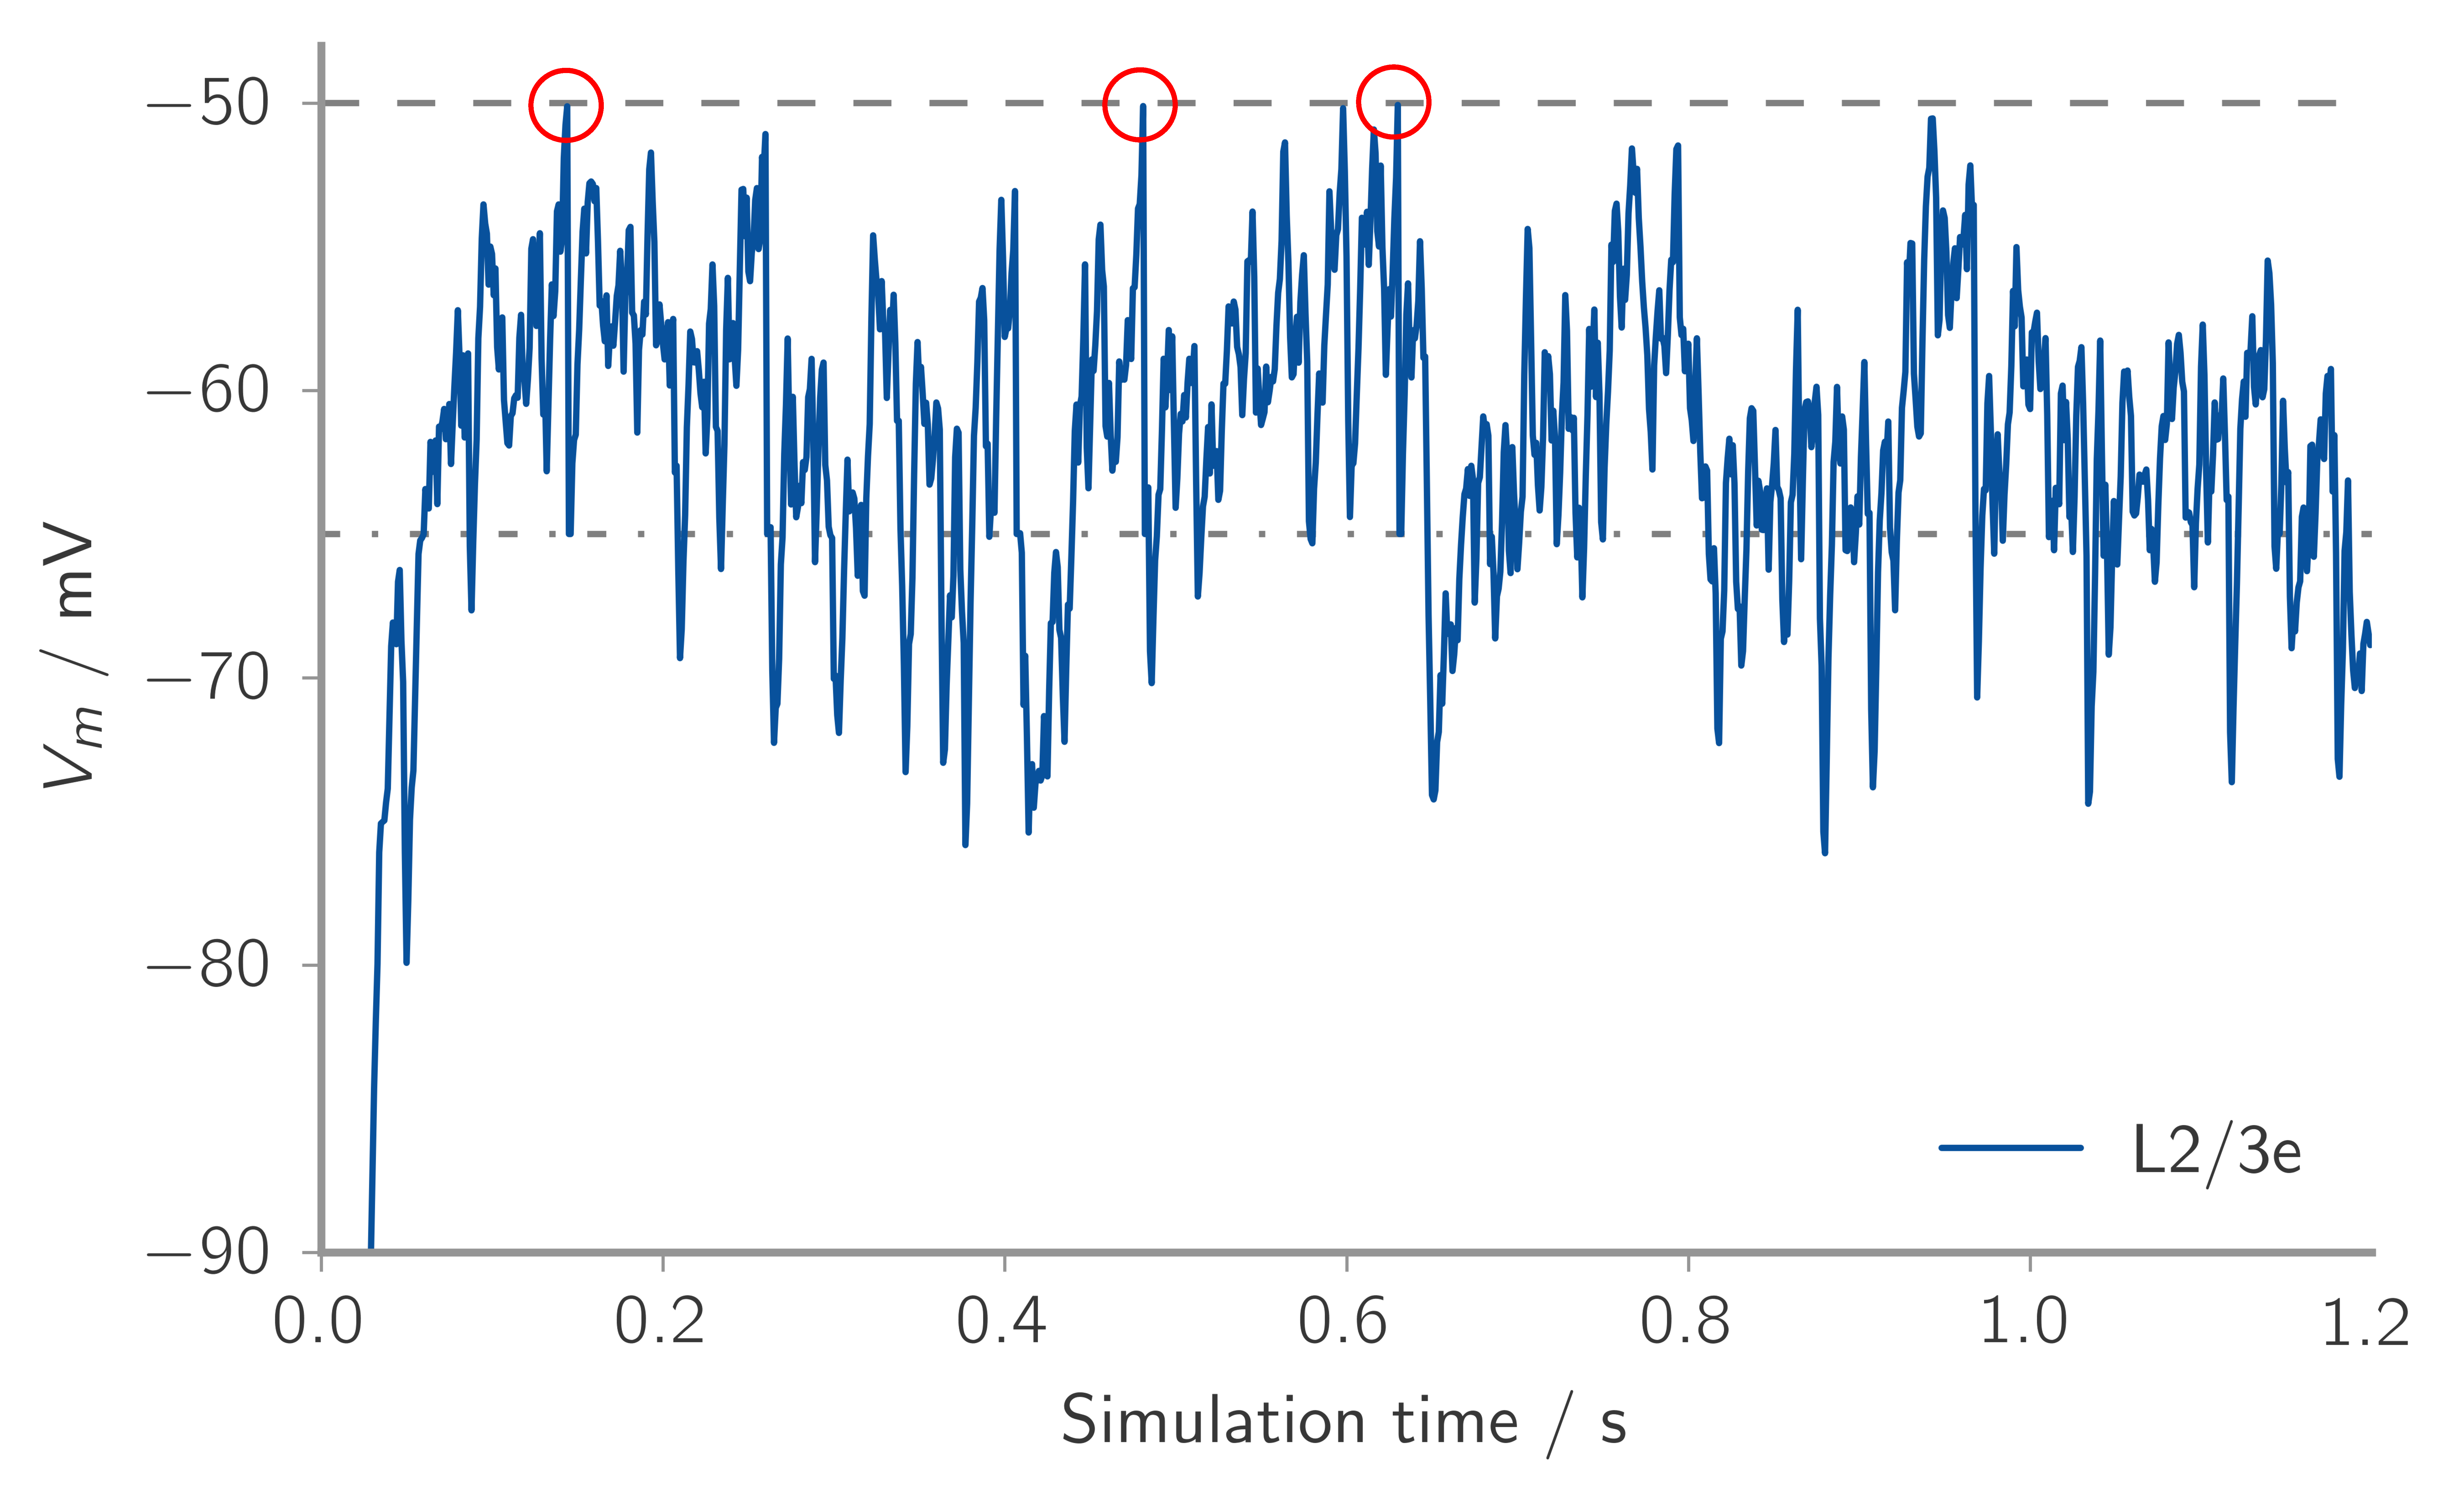
\includegraphics[height=0.8\textheight]{../figures/single_membrane_potential_spikes}
        }
        \only<3->{
            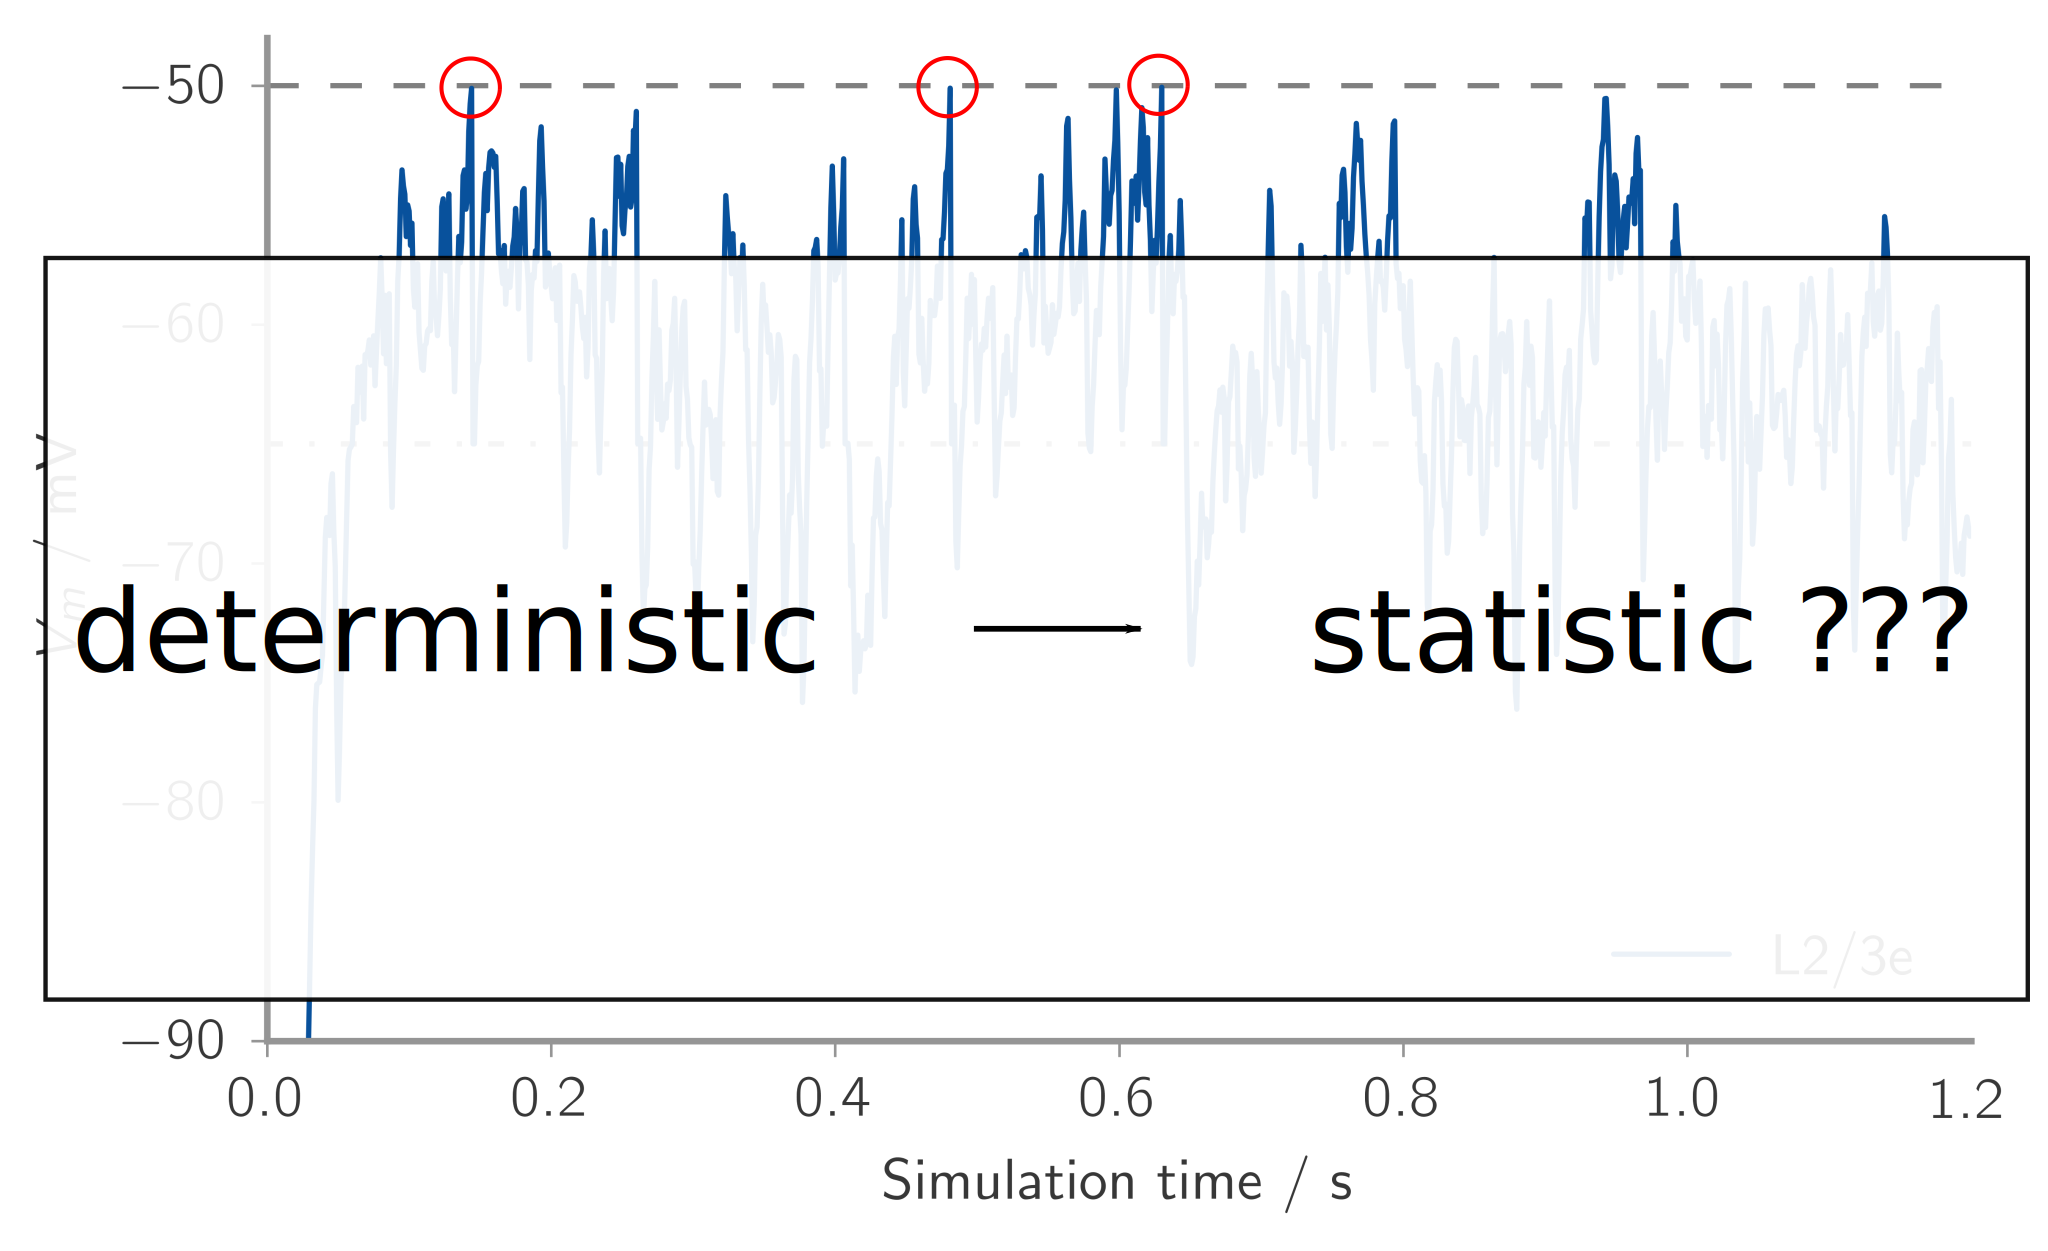
\includegraphics[height=0.8\textheight]{../figures/single_membrane_potential_spikes2}
        }
    %\end{column}
    %\begin{column}[T]{5cm} % alternative top-align that's better for graphics
        %\only<2->{
            %Distribution
            %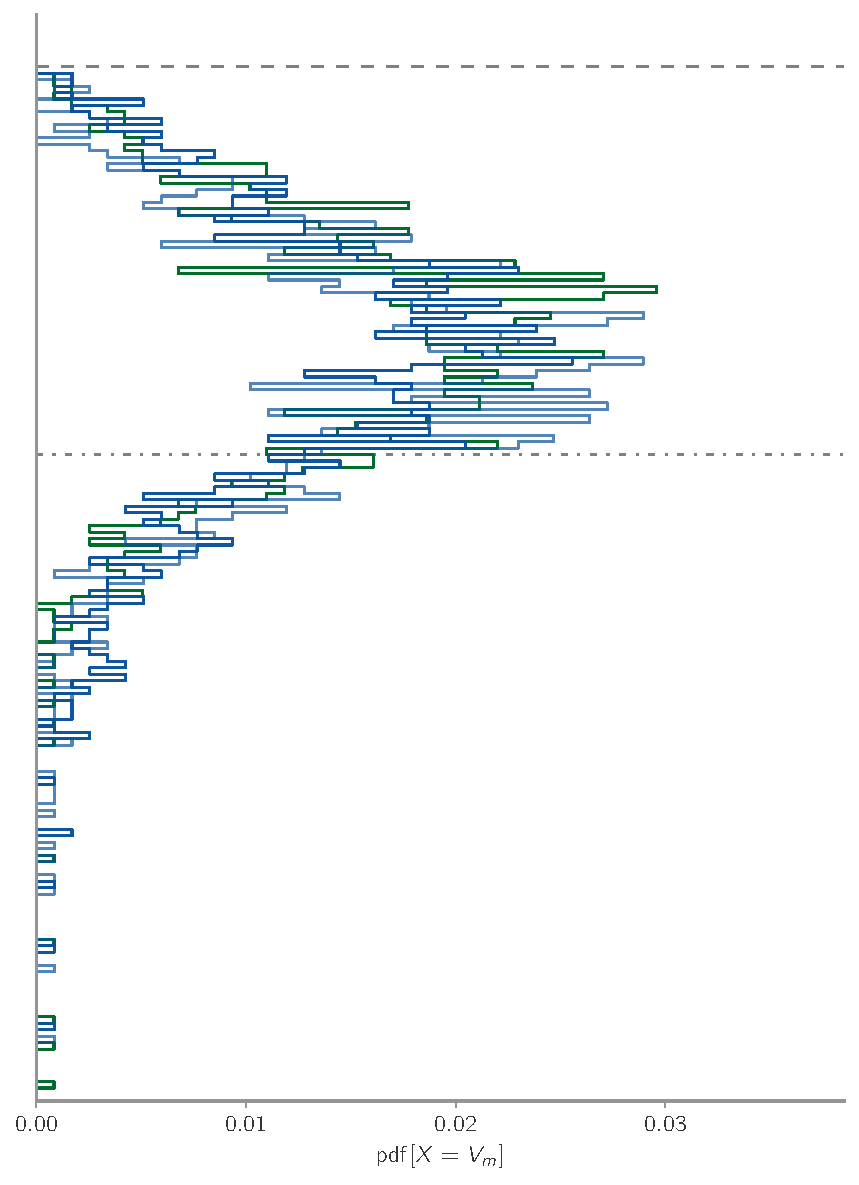
\includegraphics[height=0.7\textheight]{../figures/single_membrane_potential_distribution}
        %}
    %\end{column}
    %\end{columns}
\end{frame}


\begin{frame}[t]{Statistical description}
\only<1->{
    Sparse network: 
    \qquad $\epsilon = C / N \rightarrow 0$
}
\\
\vspace{0.8cm}
\only<2->{
    Input current:
    \begin{equation*}
        \frac{\tau_\text{m}}{C_\text{m}} \, I_i(t) = 
            \mu(t) + \sigma(t) \sqrt{\tau_\text{m}} \eta_i(t) 
    \end{equation*}
    \begin{tabular}{>{$}p{2.5cm}<{$} l}
        \mu(t)          &  Average input \\ 
        \sigma(t)       &  Amplitude of fluctuation \\
        \eta_i(t)       &  Gaussian white noise
    \end{tabular} \\
}
\vspace{0.8cm}
\only<3->{
    Uncorrelated input:
    \qquad $ \langle \eta_i(t) \: \eta_j(t') \rangle = \delta_{ij} \: \delta(t - t')$ 
}
%\vspace{0.5cm}
%\only<3->{
    %$\mu(t)$ and $\sigma^2(t)$ are linearly dependent on the firing rate $\nu(t)$ as 
    %well as the external rate $\nu_\text{ext}$.
%}
\end{frame}

\begin{frame}{}
    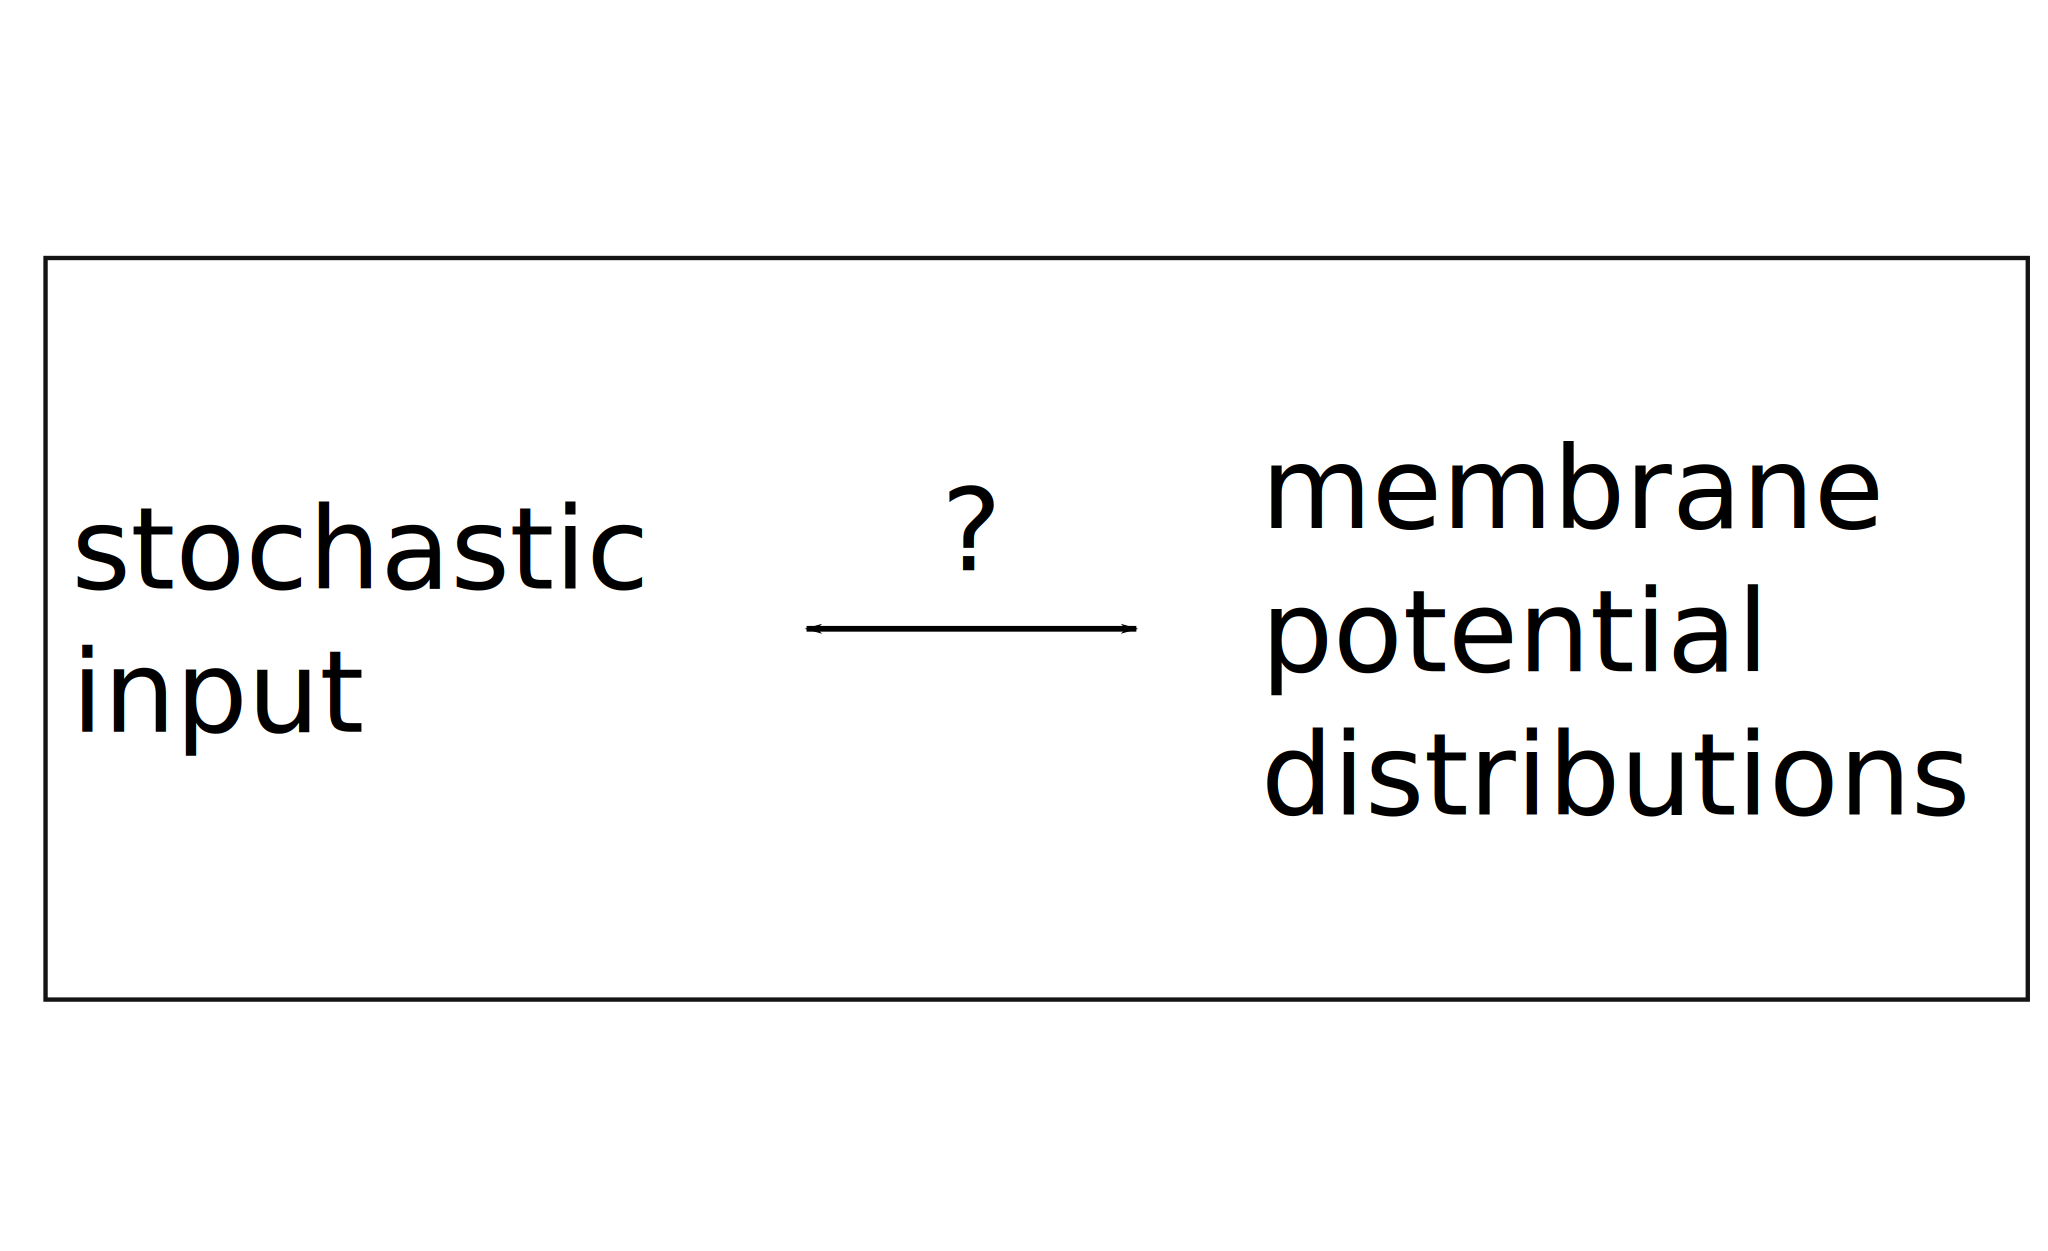
\includegraphics[height=0.8\textheight]{../figures/rate_distribution}
\end{frame}


\begin{frame}[t]{Fokker--Planck equation}
\only<1->{
    \begin{equation*}
        \tau_\text{m} \, \frac{\partial P(V, t)}{\partial t} 
           \: = \: \frac{\sigma^2(t)}{2}  \: \frac{\partial^2 P(V, t)}{\partial V^2} 
             \: + \: \frac{\partial }{\partial V}  [(V- \mu(t)) P(V, t)] 
    \end{equation*}
}
\vfill
\only<2->{
    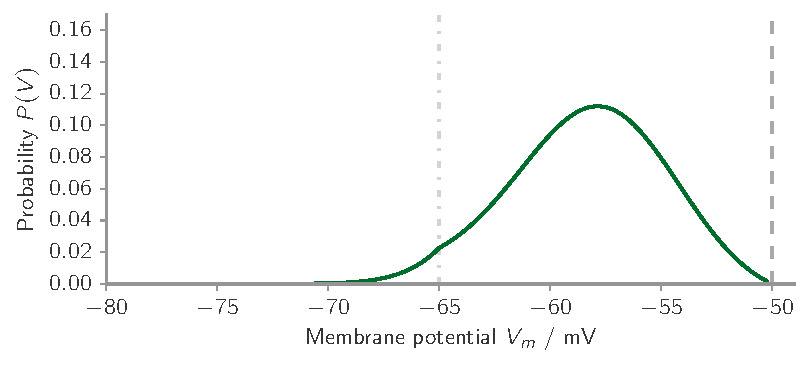
\includegraphics[height=0.6\textheight]{../figures/solution} 
}
\end{frame}

\begin{frame}[t]{Self-consistency equation}
\only<1->{
    \begin{equation*}
        \frac{1}{\nu_{a}} = \tau_{rp} 
            + \tau_\text{m} \sqrt{\pi}
                \int_{\frac{V_\text{r} - \mu_{a}}{\sigma_{a}}}^{\frac{\theta - \mu_{a}}{\sigma_{a}}} 
                    e^{u^2} \left(1 + \text{erf}(u)\right) \diff u  
    \end{equation*}
}
\vfill
\only<2->{
    Statistical input:
    \begin{align*}
        \mu_a        &= 
            \tau_\text{m} \sum_{b \,\in \,\text{pop.}} C_{ab} \, J_{ab} \, \nu_b 
            + \tau_\text{m} (C_\text{ext})_a \, J \, \nu_\text{ext} \, ; \\
        {\sigma_a}^2 &= 
            \tau_\text{m} \sum_{b \,\in \,\text{pop.}} C_{ab} \, {J_{ab}}^2  \, \nu_b
            + \tau_\text{m} (C_\text{ext})_a \,J^{\,2} \,\nu_\text{ext}
    \end{align*}
}
\end{frame}

\begin{frame}[t]{Predictions}
\only<1->{
    Firing rates $\nu_a$ \\
}
\vspace{1.5cm}
\only<2->{
    Membrane potential distribution $P_a(V)$ \\
}
\vspace{1.5cm}
\only<3->{
    Irregularity \\
     = 
    Coefficient of variation of interspike intervals
    \begin{equation*}
        \text{CV}_\text{ISI} = \frac{\sigma_\text{ISI}}{\mu_\text{ISI}} 
    \end{equation*}
}
\end{frame}



\section{Results}
\label{sec:results}

\begin{frame}[t]{Implementation of spiking network model}
    \begin{columns}[T] % contents are top vertically aligned
    \begin{column}[T]{5cm} % each column can also be its own environment
            PyNest
            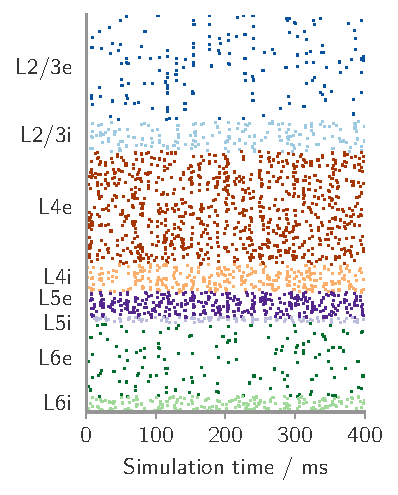
\includegraphics[width=1.0\linewidth]{../figures/raster_plot}
    \end{column}
    \begin{column}[T]{5cm} % alternative top-align that's better for graphics
            SLI
            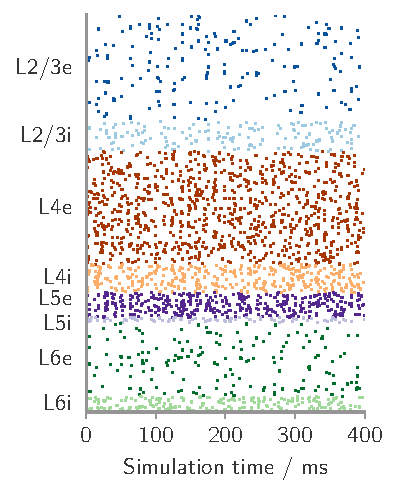
\includegraphics[width=1.0\linewidth]{../figures/raster_plot_sli}
    \end{column}
    \end{columns}
\end{frame}

\begin{frame}[t]{Statistical comparison}
    \begin{columns}[T] % contents are top vertically aligned
    \begin{column}[T]{5.0cm} % alternative top-align that's better for graphics
        \only<1->{
            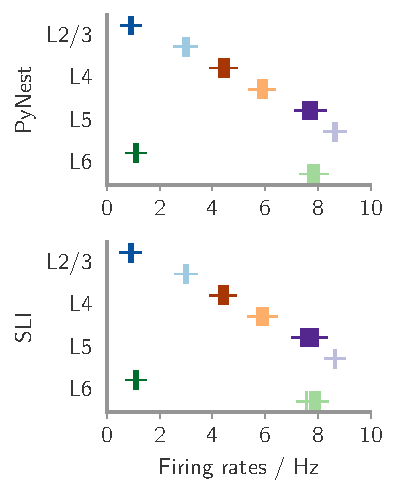
\includegraphics[height=0.8\textheight]{../figures/spon_act_rates}
        }
    \end{column}
    \begin{column}[T]{4.5cm} % alternative top-align that's better for graphics
        \only<2->{
            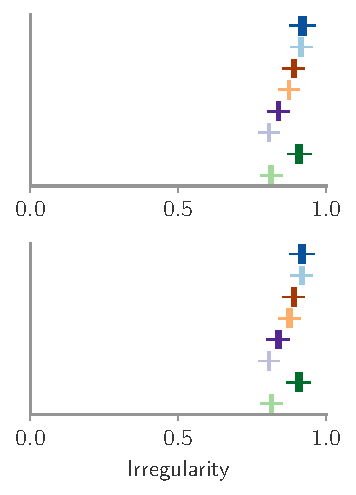
\includegraphics[height=0.8\textheight]{../figures/spon_act_irregularity}
        }
    \end{column}
    \end{columns}
\end{frame}

\begin{frame}[t]{Single neuron activity}
        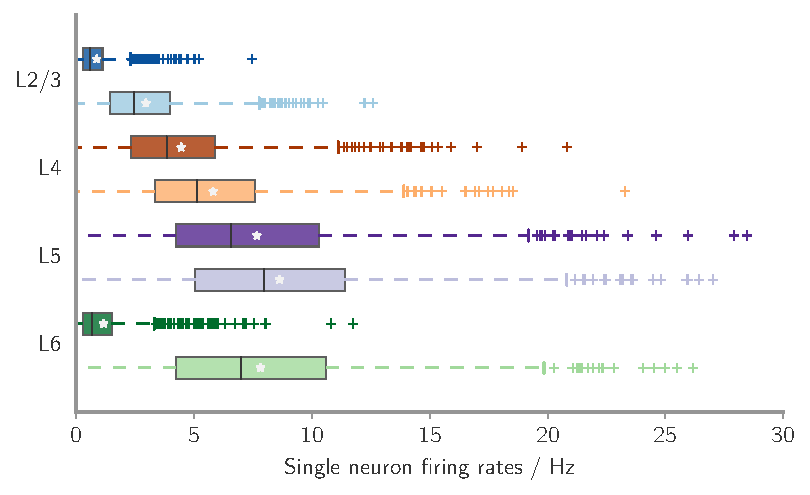
\includegraphics[height=0.8\textheight]{../figures/single_neuron_activity_rates} 
\end{frame}

\begin{frame}[t]{Mean field vs. simulation}
    \begin{columns}[T] % contents are top vertically aligned
    \begin{column}[T]{5.5cm} % each column can also be its own environment
        \only<1-1>{
        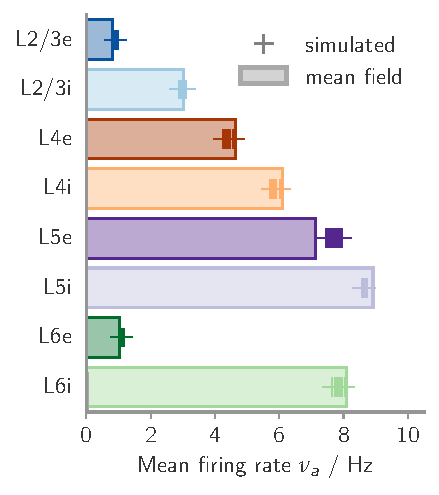
\includegraphics[height=0.7\textheight]{../figures/compare_sim_mf_fixed_total_number_rates}
        }
        \only<2-2>{
        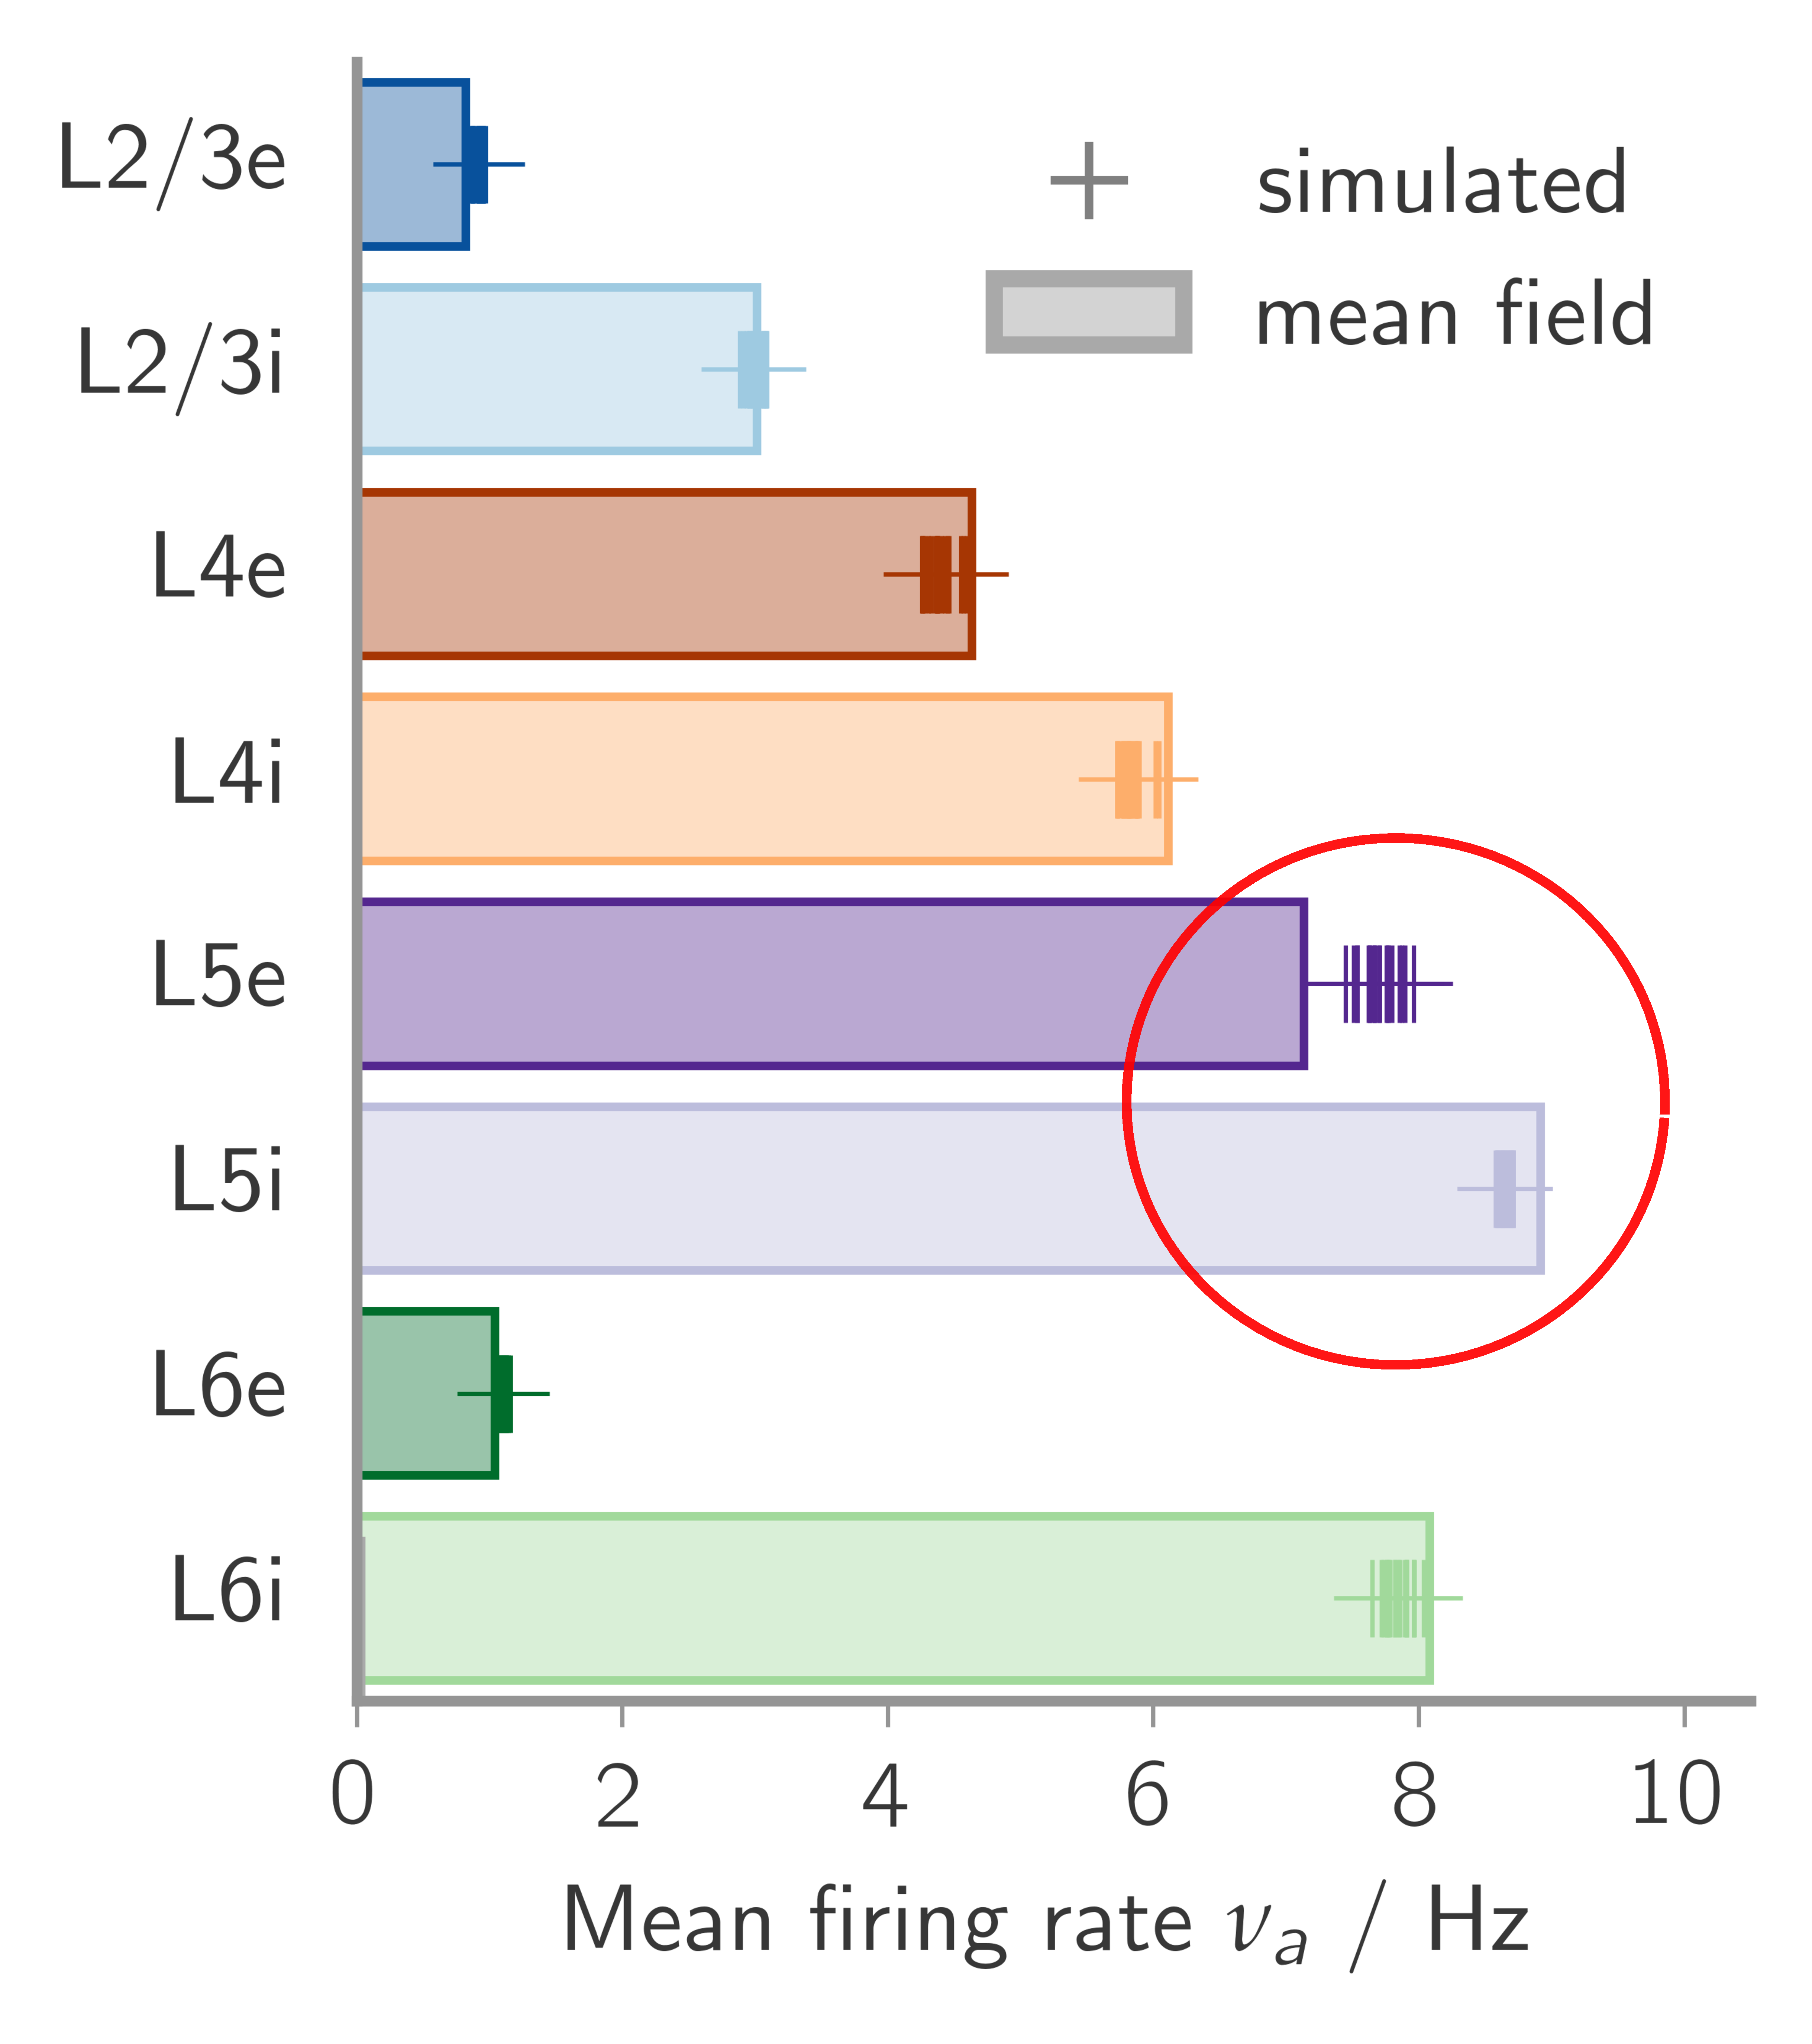
\includegraphics[height=0.7\textheight]{../figures/compare_sim_mf_fixed_total_number_rates2}
        }
        \only<3->{
        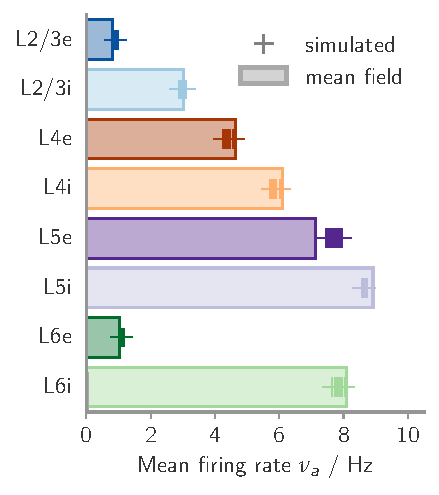
\includegraphics[height=0.7\textheight]{../figures/compare_sim_mf_fixed_total_number_rates}
        }
    \end{column}
    \begin{column}[T]{4.5cm} % alternative top-align that's better for graphics
        \only<3->{
        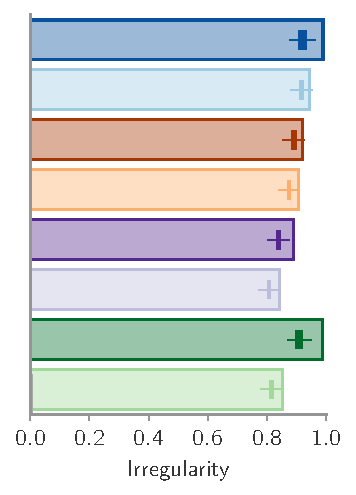
\includegraphics[height=0.7\textheight]{../figures/compare_sim_mf_fixed_total_number_irregularity}
        }
    \end{column}
    \end{columns}
\end{frame}

\begin{frame}[t]{Mean field vs. simulation}
    \center
    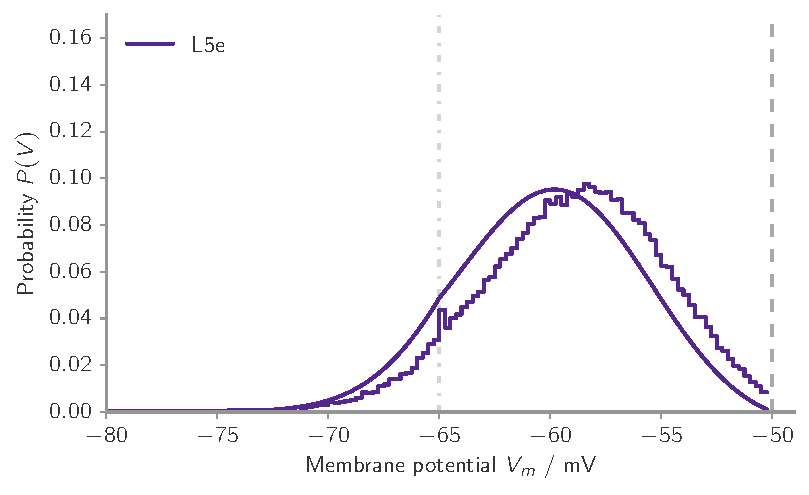
\includegraphics[height=0.8\textheight]{../figures/membrane_potential_single}
\end{frame}

\begin{frame}[t]{Applying mean field theory}
    Varying inhibitory synaptic strength $g$
    \center
    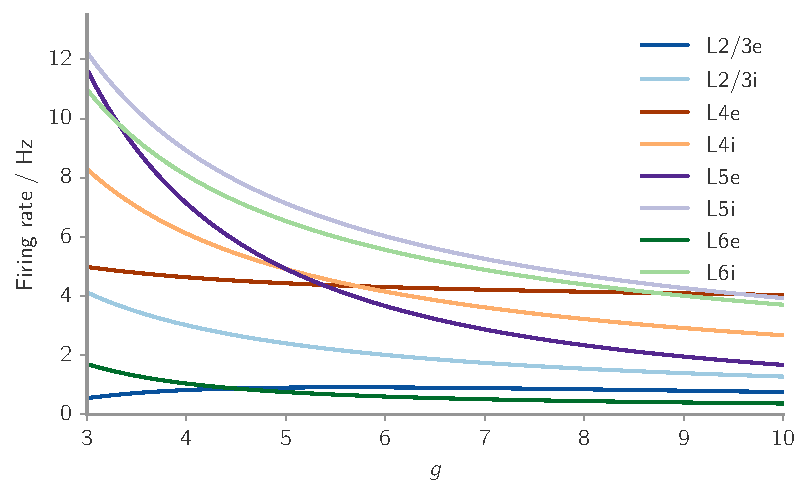
\includegraphics[height=0.7\textheight]{../figures/simulate_change_g}
\end{frame}

\section{Conclusion}
\label{sec:conclusion}

\begin{frame}[t]{Summary}
    \begin{block}<1->{Implementation successful}
        \begin{itemize}
            \item         Results of Potjans and Diesmann reproduced
        \end{itemize}
    \end{block}
    \vfill
    \begin{block}<2->{Mean field model yields good results}
        \begin{itemize}
            \item Deviations due to neglecting correlations?
        \end{itemize}
    \end{block}
    \vfill
    \begin{block}<3->{Mean field model also applicable as a tool}
        \begin{itemize}
            \item         Computationally much less expensive than simulation
        \end{itemize}
    \end{block}
\end{frame}

\begin{frame}[t]{Outlook}
    \begin{block}<1->{Extension to more distinct neuron populations}
    \end{block}
    \vfill
    \begin{block}<2->{Application to cortical computation, e.\,g. in the visual cortex}
    \end{block}
    \vfill
    \begin{block}<3->{Temporal dynamics for rate based coding}
    \end{block}
\end{frame}


\begin{frame}[t]{Acknowledgements}
    \begin{block}{Thanks to}
        \begin{itemize}
            \item Jens Timmer 
            \item Stefan Rotter
            \item Benjamin Merkt 
        \end{itemize}
    \end{block}
\end{frame}


 
\begin{frame}{}
    \huge Appendix
\end{frame}

% Population sizes
\begin{frame}[t]{Population sizes and synapse numbers}
    \begin{columns}[T] % contents are top vertically aligned
    \begin{column}[T]{5cm} % each column can also be its own environment
        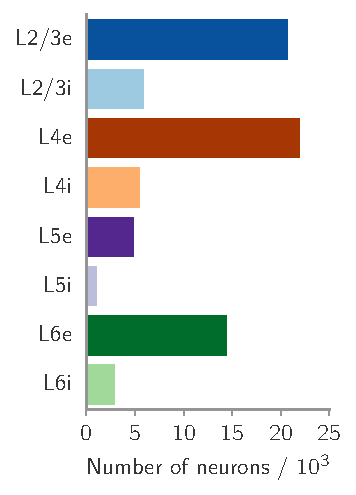
\includegraphics[width=1.0\linewidth]{../figures/population_size}
    \end{column}
    \begin{column}[T]{5cm} % alternative top-align that's better for graphics
        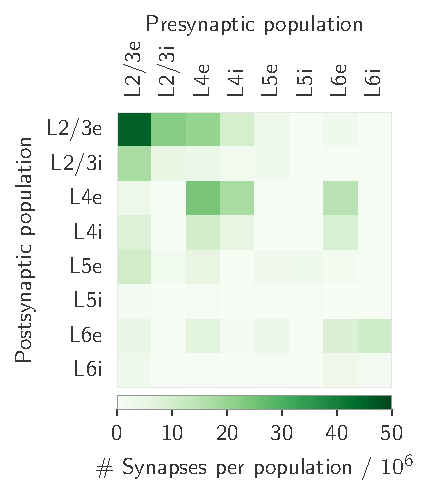
\includegraphics[width=1.1\linewidth]{../figures/synapse_numbers}
    \end{column}
    \end{columns}
\end{frame}
    

% mu and sigma in Brunel's model
\begin{frame}[t]{Single neuron firing rate in Brunel's model}
    Mean input:
\begin{equation*}
    \begin{split}
        \mu(t)          &= \mu_l(t) + \mu_\text{ext} \\
        \text{with} \qquad \mu_l(t)        &= C_E \, J (1 - \gamma g) \nu(t - d) \tau_\text{m} \\
        \text{and~~\,} \qquad \mu_\text{ext}  &= C_E J \nu_\text{ext} \tau_\text{m} \,.
    \end{split}
\end{equation*}
\vfill
    Amplitude of fluctuations:
\begin{equation*}
    \begin{split}
        \sigma^2(t)     &= {\sigma_l}^2(t) + {\sigma_\text{ext}}^2 \\
        \text{with} \qquad      {\sigma_l}^2(t)       
                        &= C_E \, J^2 (1 + \gamma g^2) \nu(t - d) \tau_\text{m} \\
            \text{and~~\,}  \qquad    
        {\sigma_\text{ext}}^2  &= C_E J^2 \nu_\text{ext} \tau_\text{m} \,.
    \end{split}
\end{equation*}
\end{frame}

% Stationary solution to Fokker--Planck equation
\begin{frame}[t]{Stationary solution}
    Constraints
\begin{align*}
    P(\theta, t) &= 0  \\
    \frac{\partial P(\theta, t)}{\partial V}    
        &= - \frac{2 \nu(t) \tau_\text{m}}{\sigma^2(t)}  \\
    \frac{\partial P(V_\text{r}^+, t)}{\partial V} \: -  \: \frac{\partial P(V_\text{r}^-, t)}{\partial V} 
        &= - \frac{2 \nu(t - \tau_\text{rp}) \tau_\text{m}}{\sigma^2(t)} \\
\lim_{V \to -\infty} P(V, t) = 0 \, ;
\quad  & \quad
    \lim_{V \to -\infty} V P(V, t) = 0 \,.
\end{align*}
    \vfill
    Solution
    \begin{equation*}
        P_0(V) = 2 \frac{\nu_0 \tau_\text{m}}{\sigma_0} 
            \exp{\left(- \frac{(V - \mu_0)^2}{{\sigma_0}^2} \right)}
            \int_{\frac{V - \mu_0}{\sigma_0}}^{\frac{\theta - \mu_0}{\sigma_0}} \! 
                \Theta \left(u - \frac{V_\text{r} - \mu_0}{\sigma_0} \right) e^{u^2} \diff u  
    \end{equation*}

\end{frame}

% Self-consistency equation -- derivation
\begin{frame}[t]{Self-consistency equation -- derivation}
    Solution
    \begin{equation*}
        P_0(V) = 2 \frac{\nu_0 \tau_\text{m}}{\sigma_0} 
            \exp{\left(- \frac{(V - \mu_0)^2}{{\sigma_0}^2} \right)}
            \int_{\frac{V - \mu_0}{\sigma_0}}^{\frac{\theta - \mu_0}{\sigma_0}} \! 
                \Theta \left(u - \frac{V_\text{r} - \mu_0}{\sigma_0} \right) e^{u^2} \diff u  
    \end{equation*} 
    \begin{equation*}
        \int_{-\infty}^{\theta} \! P_0(V) \diff V  + p_r = 1 \, ,
    \end{equation*}
    where \qquad $p_r = \nu_0 \tau_\text{rp}$. \\
\vspace{1cm}
    \begin{equation*}
        \Rightarrow \qquad
        \frac{1}{\nu_{a}} = \tau_{rp} 
            + \tau_\text{m} \sqrt{\pi}
                \int_{\frac{V_\text{r} - \mu_{a}}{\sigma_{a}}}^{\frac{\theta - \mu_{a}}{\sigma_{a}}} 
                    e^{u^2} \left(1 + \text{erf}(u)\right) \diff u  
    \end{equation*}
\end{frame}

%Backup CV of ISI predicted
\begin{frame}[t]{Predicted $P(V)$ and CV of ISI}
Membrane potential distribution:
\begin{equation*}
    P_a(V) = 2 \frac{\nu_a \tau_\text{m}}{\sigma_a} 
        \exp{\left(- \frac{(V - \mu_a)^2}{{\sigma_a}^2} \right)}
        \int_{\frac{V - \mu_a}{\sigma_a}}^{\frac{\theta - \mu_a}{\sigma_a}} \! 
            \Theta \left(u - \frac{V_\text{r} - \mu_a}{\sigma_a} \right) e^{u^2} \diff u  \,.
    \label{eq:P_V_a}
\end{equation*}
\vfill
Irregularity:
\begin{equation*}
    \text{CV}_\text{ISI}^2 
        = 2 \pi \left(\frac{\nu_a}{\tau_\text{m}}\right)^2
            \int_{\frac{V_\text{r} - \mu_{a}}{\sigma_{a}}}^{\frac{\theta - \mu_{a}}{\sigma_{a}}} 
            e^{x^2}  
            \int_{-\infty}^{x} 
            e^{u^2} \left(1 + \text{erf}(u)\right)^2 
            \diff u \, 
            \diff x 
\end{equation*}
\end{frame}

% Different synapse models
\begin{frame}[t]{Different synapse dynamics}
    Current based synapses (spiking network model):
    \begin{equation*}
        I_i(t) = 
            \sum_j w_{ij} \sum_k 
            \exp\left(\frac{t - t_j^k - d_{ij}}{\tau_\text{syn}}\right) 
    \end{equation*}
    
    \vspace{1cm}
    Voltage based synapses (mean field theory):
    \begin{equation*}
        \frac{\tau_\text{m}}{C_\text{m}} I_i(t) = 
            \tau_\text{m} \sum_j J_{ij} \sum_k \delta(t - t_j^k - d_{ij}) 
    \end{equation*}
\end{frame}

% Adaptations to mean field model: synapse model
\begin{frame}[t]{Adapting for synapse model}
\only<1->{
    Effective weight for mean input $\mu$:
    \begin{align*}
        RI_e(t)         &= 
            \frac{\tau_\text{m}}{C_\text{m}} \,w \,e^{\frac{t}{\tau_\text{m}}} 
            \qquad &\text{exponential synapse}\\
        RI_\delta(t)    &= 
            \tau_\text{m} \, J \,\delta(t)
            \qquad &\text{delta synapse}
    \end{align*}
}
\only<2->{
    Matching the kernels (with $k_e(t) = e^{\frac{t}{\tau_\text{m}}}$):
    \begin{equation*}
        \int_{0}^{\infty}\delta(t)\diff t 
            = 1 
            = \int_{0}^{\infty} a_\mu k_e(t)\diff t  
            = a_\mu \tau_\text{s} 
    \end{equation*}
}
\only<3->{
    Matching the synapses:
    \begin{align*}
        \int_{0}^{\infty} \tau_\text{m} \,J \,a_\mu\, k_e(t) \diff t 
            &= \int_{0}^{\infty} \frac{\tau_\text{m} }{C_\text{m}} \,w\, k_e(t)\diff t  \\
        \Rightarrow \qquad
        J   &= \frac{w \, \tau_\text{s}}{C_\text{m}} 
    \end{align*}
}
\end{frame}

\begin{frame}[t]{Adapting for synapse model}
Effective weight for fluctuations $\sigma^2(t)$
\only<1->{
    Matching squared kernels:
    \begin{align*}
        1   &= {a_\sigma}^2 \int_{0}^{\infty}(k_e(t))^2\diff t  \\
            &= {a_\sigma}^2 \, \frac{\tau_\text{s} }{2} \\
    \Rightarrow \qquad
    {a_\sigma}^2 &= 2 / \tau_\text{s} 
    \end{align*}
}
\only<2->{
    Matching squared synapses:
    \begin{align*}
    \int_{0}^{\infty} \left(\tau_\text{m} \,J \,a_\sigma\, k_e(t)\right)^2 \diff t 
        &= \int_{0}^{\infty} 
        \left(\frac{\tau_\text{m} }{C_\text{m}} \,w\, k_e(t)\right)^2\diff t 
    \\
    \Rightarrow \qquad
    {J_\text{eff}}^2 
        &=  \frac{w^2}{{C_\text{m}}^2} \,\frac{\tau_\text{s} }{2}  
    \end{align*}
}
\end{frame}


\begin{frame}[t]{Adapting for synapse model}
Resulting equation for $\mu_a$ and $\sigma_a$:
\begin{align*}
    \mu_a        &= 
        \sum_{b \,\in \,\text{pop.}}  (M_\text{local})_{ab} \: \nu_b 
        + (M_\text{ext})_{a} \: \nu_\text{ext} \, ; \\
    {\sigma_a}^2 &= 
        \sum_{b \,\in \,\text{pop.}} (S_\text{local})_{ab} \: \nu_b
        + (S_\text{ext})_{a}  \:\nu_\text{ext}\,.
\end{align*}
where
\begin{align*}
    (M_\text{local})_{ab} 
        &:= \tau_\text{m} \, C_{ab} \,J_{ab} \,;\\ 
    (M_\text{ext})_{a} 
        &:= \tau_\text{m} \, (C_\text{ext})_a \,J \,;\\
    (S_\text{local})_{ab} 
        &:= \tau_\text{m} \,(1 + {\Delta_J}^2) \,C_{ab} \,({J_\text{eff}}^2)_{ab} \,;\\
    (S_\text{ext})_{a} 
        &:= \tau_\text{m} \,(1 + {\Delta_J}^2) \,(C_\text{ext})_a \,{J_\text{eff}}^2 
\end{align*}
\end{frame}

% Comparing synchrony
\begin{frame}[t]{Comparing synchrony}
    \begin{columns}[T] % contents are top vertically aligned
    \begin{column}[T]{5.5cm} % alternative top-align that's better for graphics
        \only<1->{
            Synchrony = Fano factor ($\frac{\sigma^2}{\mu}$) of PSTH
        }
    \end{column}
    \begin{column}[T]{4.5cm} % alternative top-align that's better for graphics
        \only<2->{
            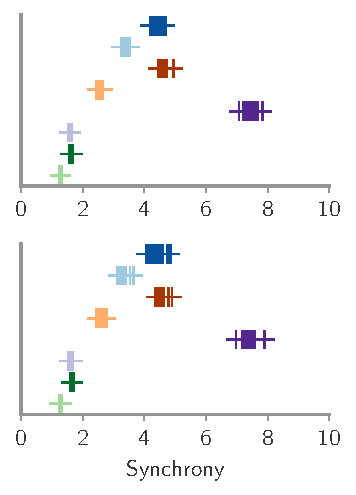
\includegraphics[height=0.8\textheight]{../figures/spon_act_synchrony}
        }
    \end{column}
    \end{columns}
\end{frame}


    
\end{document}
